\subsection{DCGAN}

Generative Adversarial Networks (GANs) are a class of machine learning frameworks introduced by Goodfellow et al. in 2014 \cite{goodfellow2014}. GANs have revolutionized the field of generative modeling, allowing for the creation of highly realistic synthetic data. This section will explore the fundamental concepts, structure, and applications of Deep Convolutional Generative Adversarial Networks (DCGANs).

\subsubsection{Introduction to DCGANs}

DCGANs consist of two neural networks: the generator and the discriminator, which compete to minimize their respective loss functions. The generator aims to create data that is indistinguishable from real data, while the discriminator attempts to differentiate between real and generated data. This adversarial process continues until the generator produces data that the discriminator cannot reliably distinguish from real data. DCGANs leverage convolutional neural networks (CNNs) to improve the quality of generated images.

\begin{figure}[H]
    \centering
    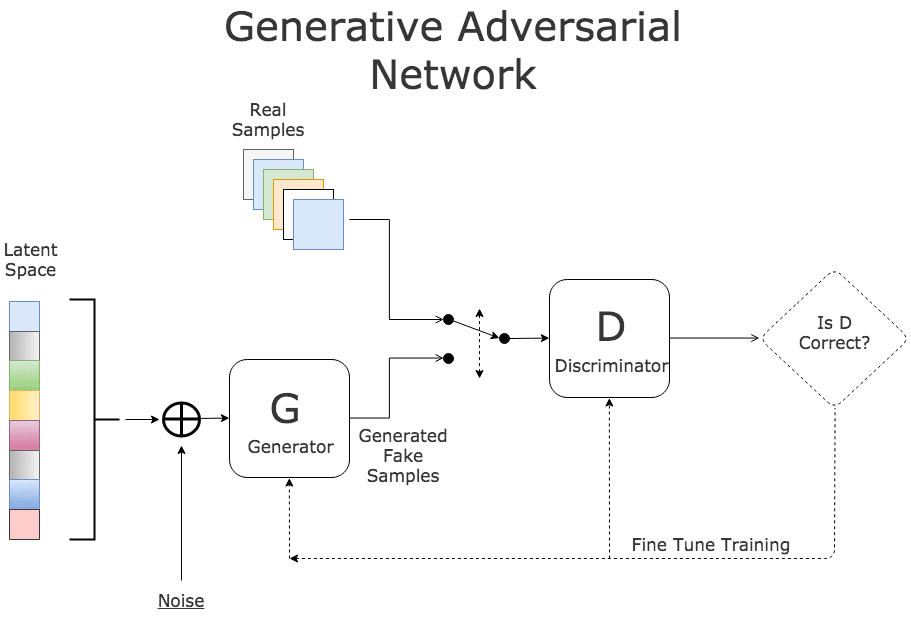
\includegraphics[width=0.6\textwidth]{assets/gan_structure.png}
    \caption{Structure of a Generative Adversarial Network, picture from \cite{kdnuggets2017}}
    \label{fig:gan_structure}
\end{figure}

\subsubsection{Components of DCGANs}

The two primary components of DCGANs are:

\paragraph{Generator}
\hfill \break
The generator, \( G \), is a convolutional neural network that takes random noise, \( z \), from a latent space and transforms it into a synthetic data sample, \( G(z) \). The objective of the generator is to produce data that is as close as possible to the real data distribution. The generator's loss function is designed to minimize the likelihood of the discriminator correctly identifying the generated data as fake.
\\
The actual structure of the generator, inspired by the standard DCGAN presented in \cite{radford2016}:

\begin{figure}[h]
    \centering
    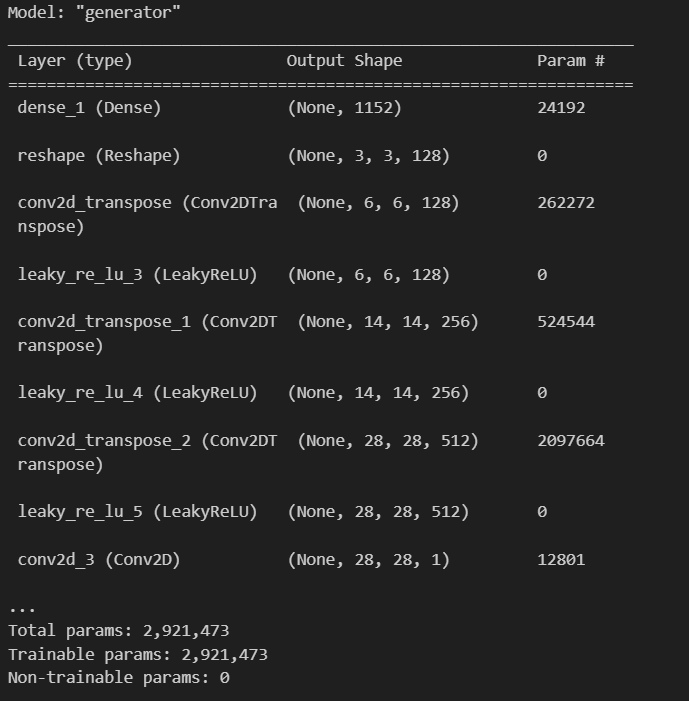
\includegraphics[width=0.7\textwidth]{assets/Generator.png}
    \caption{Structure of a Deep Convolutional Generative Adversarial Network Generator}
    \label{fig:gan_generator_structure}
\end{figure}

\paragraph{Discriminator}
\hfill \break
The discriminator, \( D \), is another convolutional neural network that evaluates data and assigns a probability that a given sample comes from the real data distribution rather than the generator. The discriminator's loss function aims to maximize the likelihood of correctly classifying real and fake data.
\\
The actual structure of the discriminator, inspired by the standard DCGAN presented in \cite{radford2016}:

\begin{figure}[h]
    \centering
    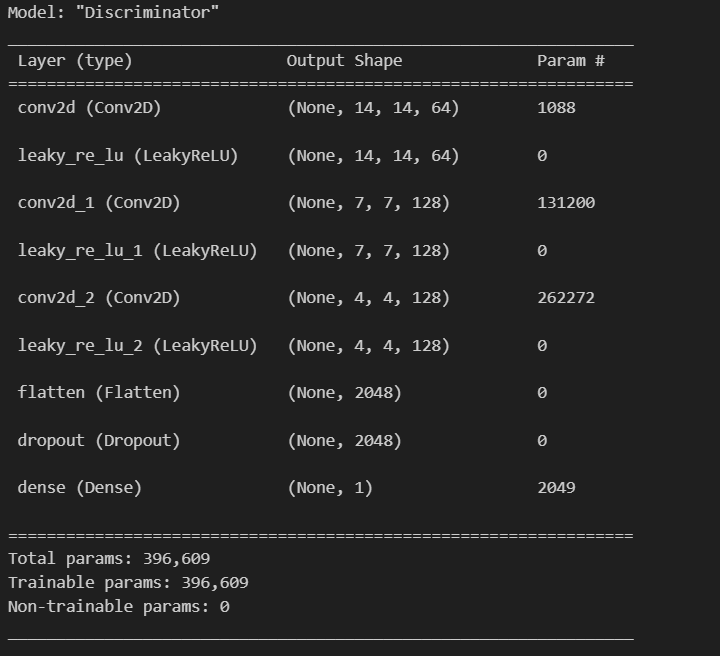
\includegraphics[width=0.7\textwidth]{assets/Discriminator.png}
    \caption{Structure of a Deep Convolutional Generative Adversarial Network Discriminator}
    \label{fig:gan_disciminator_structure}
\end{figure}

\subsubsection{Training Process}

The training process for DCGANs involves optimizing the following value function, \( V(G, D) \), which is a minimax game between \( G \) and \( D \):
\begin{equation}
\min_G \max_D V(G, D) = \mathbb{E}_{\mathbf{x} \sim p_\text{data}(\mathbf{x})} [\log D(\mathbf{x})] + \mathbb{E}_{\mathbf{z} \sim p_\mathbf{z}(\mathbf{z})} [\log (1 - D(G(\mathbf{z})))]
\end{equation}
The training of DCGANs involves alternating between updating the discriminator and the generator. The discriminator is trained to maximize its classification accuracy, while the generator is trained to deceive the discriminator. This iterative process can be summarized in the following steps:

\begin{enumerate}
    \item Sample a batch of real data and a batch of random noise.
    \item Update the discriminator by maximizing its loss function with both real and generated data.
    \item Sample a new batch of random noise.
    \item Update the generator by minimizing its loss function, which depends on the discriminator's performance.
\end{enumerate}


